%---------------------------------------------------------------------------%
%-                                                                         -%
%-                           LaTeX Template                                -%
%-                                                                         -%
%---------------------------------------------------------------------------%
%- Copyright (C) Huangrui Mo <huangrui.mo@gmail.com> 
%- This is free software: you can redistribute it and/or modify it
%- under the terms of the GNU General Public License as published by
%- the Free Software Foundation, either version 3 of the License, or
%- (at your option) any later version.
%---------------------------------------------------------------------------%
%->> Document class declaration
%---------------------------------------------------------------------------%
\documentclass[twoside]{Style/ucasthesis}%
%- Multiple optional arguments:
%- [<oneside|twoside|print>]% oneside eprint, twoside eprint, or paper print
%- [fontset=<adobe|none|...>]% specify font set instead of automatic detection
%- [scheme=plain]% thesis writing of international students
%- [draftversion]% show draft version information
%- [standard options for ctex book class: draft|paper size|font size|...]%
%---------------------------------------------------------------------------%
%->> Document settings
%---------------------------------------------------------------------------%
\usepackage[numbers,list]{Style/artratex}% 文本: Jones [1]; 括号: [1] document settings
%- usage: \usepackage[option1,option2,...,optionN]{artratex}
%- Multiple optional arguments:
%- [bibtex|biber]% set bibliography processor and package
%- [<numbers|super|authoryear|alpha>]% set citation and reference style
%- <numbers>: textual: Jones [1]; parenthetical: [1]
%- <super>: textual: Jones superscript [1]; parenthetical: superscript [1]
%- <authoryear>: textual: Jones (1995); parenthetical: (Jones, 1995)
%- <alpha>: textual: not available; parenthetical: [Jon95]
%- [geometry]% reconfigure page layout via geometry package
%- [lscape]% provide landscape layout environment
%- [xhf]% disable header and footer via fancyhdr package
%- [color]% provide color support via xcolor package
%- [background]% enable page background
%- [tikz]% provide complex diagrams via tikz package
%- [table]% provide complex tables via ctable package
%- [list]% provide enhanced list environments for algorithm and coding
%- [math]% enable some extra math packages
%- [xlink]% disable link colors
\usepackage{Style/artracom}% user defined commands
%---------------------------------------------------------------------------%
%->> Document inclusion
%---------------------------------------------------------------------------%
%\includeonly{Tex/Chap_1,...,Tex/Chap_N}% selected files compilation
%---------------------------------------------------------------------------%
%->> Document content
%---------------------------------------------------------------------------%
%-
%-> Titlepage information
%-
%---------------------------------------------------------------------------%
%->> Titlepage information
%---------------------------------------------------------------------------%
%-
%-> 中文封面信息
%-
\confidential{}% 密级:只有涉密论文才填写
\schoollogo[scale=1]{logo}% 校徽
\title{基于Flask的可视化COVID-19疫情数据监测平台}% 论文中文题目
\author{刘浩鑫}% 论文作者
\advisor{王震}% 指导教师:姓名 专业技术职务 工作单位
%\advisor{指导教师一\\指导教师二\\指导教师三}% 多行指导教师示例
\degree{论文}% 学位:学士、硕士、博士
\degreetype{学年}% 学位类别:理学、工学、工程、医学等
\major{信息与计算科学}% 二级学科专业名称
\institute{内蒙古大学~数学科学学院}% 院系名称
\date{2021~年~9~月}% 毕业日期:夏季为6月、冬季为12月
%-
%-> 英文封面信息
%-
\TITLE{Visual COVID-19 epidemic data monitoring platform based on Flask and MySQL}% 论文英文题目
\AUTHOR{Liu Haoxin}% 论文作者
\ADVISOR{Supervisor: Associate Professor Wang Zhen}% 指导教师
\DEGREE{Bachelor}% 学位:Bachelor, Master, Doctor, Postdoctor。封面据英文学位名称自动切换,需确保拼写准确
\DEGREETYPE{Natural Science}% 学位类别:Philosophy, Natural Science, Engineering, Economics, Agriculture 等
\MAJOR{Information and Computing Sciences}% 二级学科专业名称
\INSTITUTE{Department of mathmatics, Inner Mongolia University}% 院系名称
\DATE{September, 2021}% 毕业日期:夏季为June、冬季为December
%---------------------------------------------------------------------------%
%
\begin{document}
%-
%-> Frontmatter: title page, abstract, content list, symbol list, preface
%-
\frontmatter% initialize the environment
%---------------------------------------------------------------------------%
%->> Frontmatter
%---------------------------------------------------------------------------%
%-
%-> 生成封面
%-
\maketitle% 生成中文封面
\MAKETITLE% 生成英文封面
%-
%-> 作者声明
%-
% \makedeclaration% 生成声明页
%-
%-> 中文摘要
%-
\intobmk\chapter*{摘\quad 要}% 显示在书签但不显示在目录
\setcounter{page}{1}% 开始页码
\pagenumbering{Roman}% 页码符号

自2019年末一种新型冠状病毒(COVID-19)在我国武汉被发现以来,人们的日常生活收到了极大的影响。昔日车水马龙的街道上冷冷清清,再也没有以往的欢声笑语。这样的环境给我们带来了恐慌,因此疫情数据的监测与预测也越来越显得重要。及时、准确的疫情数据对于国家政策的制定、社会的经济发展具有十分重要的意义。

此平台以腾讯疫情数据网站所公布各省市、国内外疫情数据作为研究对象,使用Python爬取数据并将数据存储于MySQL数据库中,然后使用Flask技术将数据可视化展现在面板中以供监测,并提供累计确诊地图、新增确诊病例地图。

\keywords{Python,Flask,COVID-19,数据可视化,MySQL}% 中文关键词
%-
%-> 英文摘要
%-
\intobmk\chapter*{Abstract}% 显示在书签但不显示在目录

Since the end of 2019, a New Coronavirus (COVID-19) was discovered in Wuhan, China, and people's daily life has been greatly affected. The busy streets of the past were deserted, without the laughter of the past. Such an environment has brought us panic, so the monitoring and prediction of epidemic data is becoming more and more important. Timely and accurate epidemic data is of great significance for the formulation of national policies and social and economic development.

This platform takes the epidemic data of provinces and cities, domestic and foreign countries published by Tencent epidemic data website as the research object, uses Python to crawl the data and store the data in MySQL database, then uses flask technology to visualize the data in the panel for monitoring, and provides cumulative confirmed map and new confirmed case map.

\KEYWORDS{Python, Flask, COVID-19, Data Visualization, MySQL}% 英文关键词
%---------------------------------------------------------------------------%% title page, abstract
{% content list region
\linespread{1.2}% local line space
\intobmk*{\cleardoublepage}{\contentsname}% add link to bookmark
\tableofcontents% content catalog
\intobmk*{\cleardoublepage}{\listfigurename}% add link to bookmark
\listoffigures% figure catalog
% \intobmk*{\cleardoublepage}{\listtablename}% add link to bookmark
% \listoftables% table catalog
}
% \input{Tex/Prematter}% symbol list, preface content
%-
%-> Mainmatter
%-
\mainmatter% initialize the environment
%---------------------------------------------------------------------------%
%->> Main content
%---------------------------------------------------------------------------%
\chapter{绪论}

\section{研究背景与意义}

\subsection{研究背景}

目前,世界仍在与新冠病毒作斗争,世界正处于大变革、大调整和两极分化的转折点。从目前疫情来看,即使一些国家实现了所谓的“群体免疫”,但除中国、韩国、朝鲜和新西兰等少数国家外,大多数国家的社会开放和经济重启计划仍远未达到预期。一些医学专家甚至断言,COVID-19将与人类长期共存。在此之前,由于中美之间的结构性竞争和贸易摩擦,全球经济地理空间重组。COVID-19的爆发无疑加剧了中美之间固有的差异。疫情发生后,世界格局将迎来新一轮深刻调整,世界新秩序正在全球抗击疫情的斗争中悄然孕育。展望未来,以开放、包容、协作和协商为特征的全球安全进程可能会突然结束,取而代之的是全球供应链和产业链的中断、国家间人员交流的限制性孤立以及各种种族主义和仇外心理的抬头。在新的政治形势和新的技术环境下,大数据被广泛应用于新冠疫情防控和社会稳定监测。以新冠疫情防控为契机,以精准安全管理为目标,以大数据为核心动力,全球安全管理人工智能时代正在悄然开启。

2020年2月,世卫组织总干事谭德塞在记者会上宣布,将新型冠状病毒命名为“COVID-19”。据国家卫生委员会统计,截止2021年8月7日,我国31个省(区、市)和新疆建设兵团累计确诊病例121454例,累计死亡5654人;国外累计确诊病例202337884,累计死亡4285250人。我国国内确诊病例数仍呈现上升趋势,可见当前国内疫情形势仍然相当严峻。


\subsection{研究意义}

新型冠状病毒肺炎疫情在 2019 年底爆发,并迅速在全球范围内传播。疫情发展实况与每个人的工作和生活息息相关。同时,网络上也出现了疫情相关的虚假信息和谣言,扰乱了社会防疫抗疫秩序。基于爬虫编程技术实现了对新冠疫情数据的采集,通过疫情数据可视化,将国内外疫情形态以更直观的方式传递给大众,帮助人们更好地了解国内外疫情实况,提高防范意识,从而有效地协调、安排和开展各项工作和生活等。本系统使用Flask框架、Python构建轻量级疫情数据发布平台,将疫情数据转换为可视化的地图与表格,最大程度上满足疫情时代下人们的普遍需求。本文将从疫情数据的获取及存储、网页设计等几个方面进行阐述。\citep{李宏2020基于民众视阈下的疫情数据可视化设计路径研究}

2020年初,新型冠状病毒肺炎疫情已成为世界焦点,从疫情初现端倪,政府和企业在此次疫情中的数据可视化,让公众直观地掌握疫情动态。达到防控风险,抑制疫情的再扩散的目的。当今世界已经进入大数据时代,各国已将数据列为新的战略资源。在经济高速运转的今天,数据不再局限于小小的一个圈子,而是更加开放、包容,数据规模也更为客观。数据不再是简单的数字,如何从数据的背后挖掘出数据潜藏的价值成为国家和企业关心的热点问题。\citep{郭宏曦2020新型冠状病毒肺炎疫情数据的可视化探索}

\section{国外研究现状}

针对全球流行的新型冠状病毒,Google新闻推出基于维基百科以及其他数据来源的疫情数据监测平台。世卫组织(WHO)也在其官网发布疫情数据以及预防感染措施,以减少人们对新冠病毒的恐惧。

\begin{figure}[H]
    \centering
    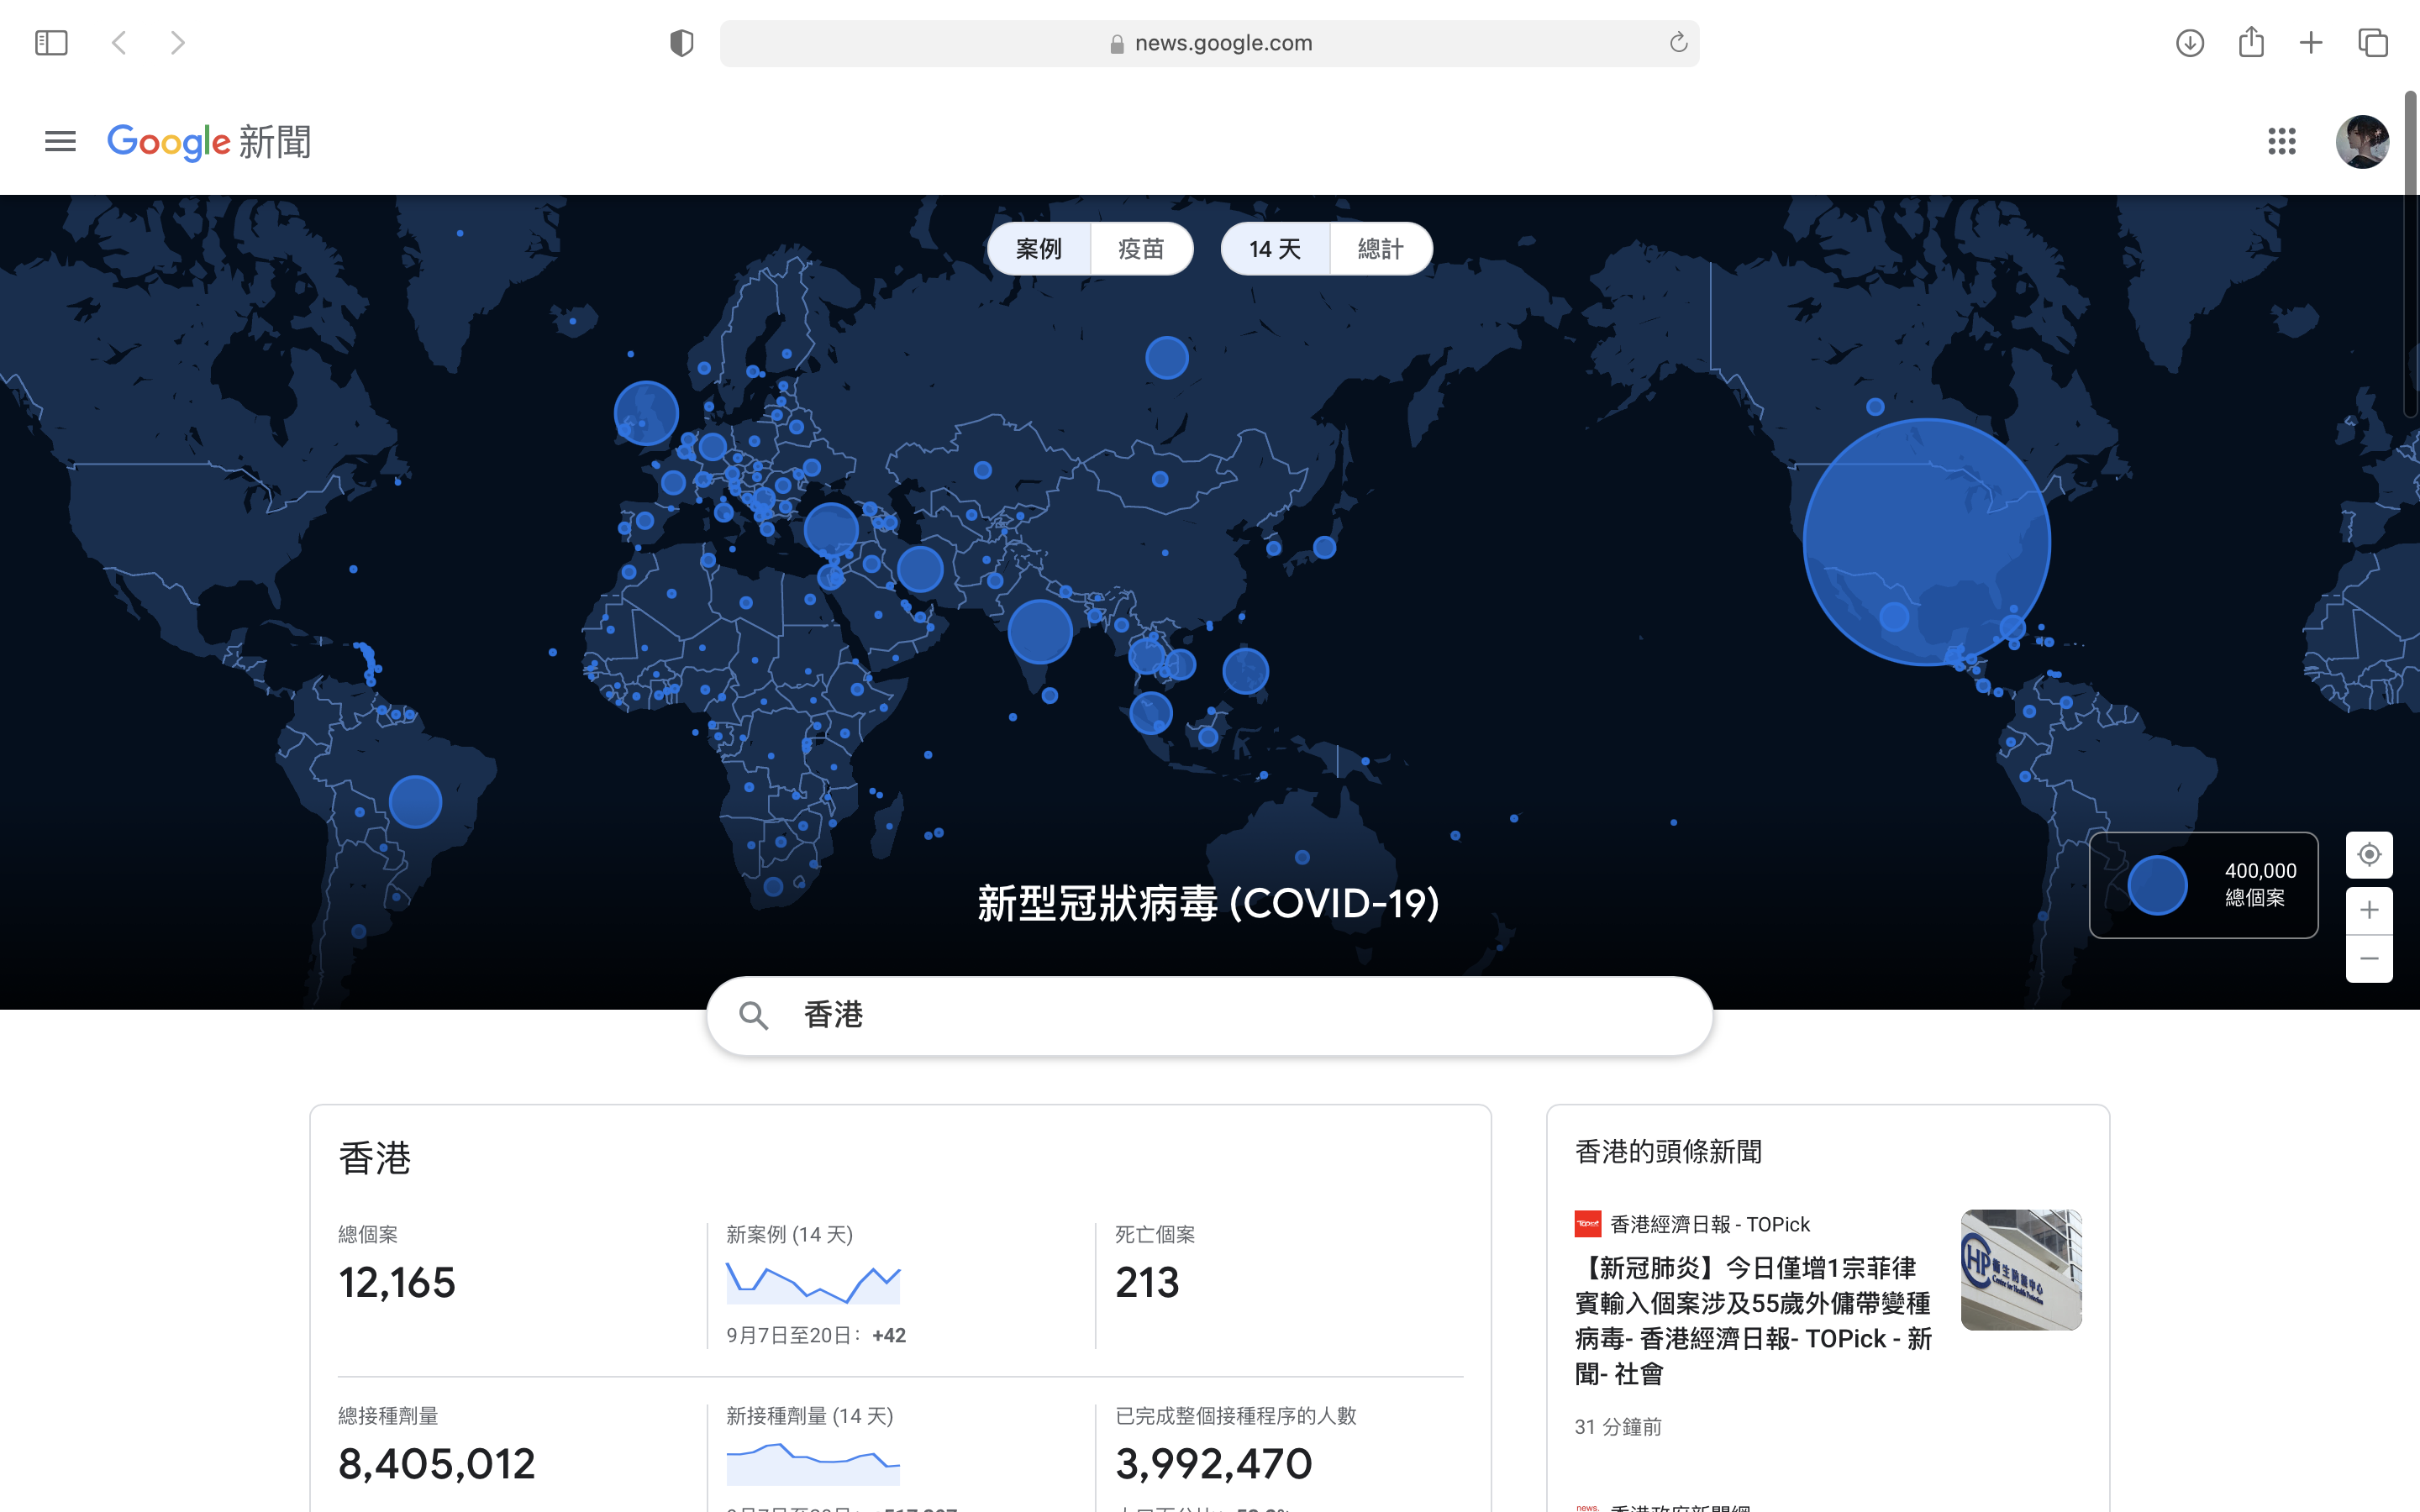
\includegraphics[width=0.8\textwidth]{t1}
    \bicaption{谷歌新闻疫情数据监测网站}{Google News epidemic data monitoring website}
    \label{fig:t1}
\end{figure}

\section{研究方法}

由于时间和精力的限制,本系统采用的疫情原始数据来自于阿里巴巴、腾讯或百度等已有疫情数据平台的数据源,而不再去统计疫情数据。

在现实生活中,单纯的数字不能直观地显示一段时间以来的发展状况,并且人脑对图像信息的处理能力也要优于对单纯数据的处理,所以将数据可视化更有利于普通大众更快地获取信息。同时,数据可能是多维度的,将数据按照一定规则分类、排序可视化之后更能清楚地看到数据的多维性,更能表达出数据与数据之间的关系。当前的数据可视化的系统设计方法有多种,但是主要的设计方法还是设计前端+后端+数据库的主体思路。\citep{韩洪勇2020基于}

基于Python+Echarts的大数据可视化系统采用B/S架构,借助于Python强大的数据获取和处理技术实现了区域网络餐饮数据的采集、清洗、整理及分析计算工作并推送至MySQL数据库中。后台采用基于Python的Flask框架实现数据接口功能,前端综合运用了HTML、CSS、JavaScript等,并结合Echarts数据可视化组件,实现了数据到可视化图表的转换。\citep{陈俊生2019基于}


\chapter{开发环境及其简介}
\section{开发环境}

以下为开发环境列表
\begin{center}
  \begin{tabular}{lcc}
    \hline
    开发环境 & 名称 & 版本 \\
    \hline
    开发系统 & macOS Big Sur & 11.5.1\\
    IDE & PyCharm & 2021.2\\
    前端 & Vscode & 1.60.1 (Universal)\\
    Python & Python & 3.7.1\\
    Python依赖 & flask, requests, pymysql &  --- \\
    数据库 & MySQL & 8.0.26 Homebrew\\
    \hline
  \end{tabular}
\end{center}

\section{开发环境简介}

% \begin{figure}[htbp]
%   \centering
%   \includegraphics[height=6.0cm,width=9.5cm]{Img/t2.png}%fig2文件夹下的xbee.esp图片,
%   \caption{Campus environment detection system}
% \end{figure}
Flask是一个使用 Python 编写的轻量级 Web 应用框架,包括Werkzeug和Jinja2两个核心函数库,它们分别负责业务处理和安全方面的功能,这些基础函数为web项目开发过程提供了丰富的基础组件。。其 WSGI 工具箱采用 Werkzeug ,模板引擎则使用 Jinja2 ,Flask使用 BSD 授权。Flask的基本模式为在程序里将一个视图函数分配给一个 URL,每当用户访问这个URL时,系统就会执行给该URL 分配好的视图函数,获取函数的返回值并将其显示到浏览器上,其工作过程如下所示。\citep{grinberg2018flask}

\begin{figure}[H]
  \centering
  \includegraphics[width=0.8\textwidth]{t2}
  \bicaption{Flask工作流程}{Flash workflow}
  \label{fig:t2}
\end{figure}


默认情况下,Flask 不包含数据库抽象层、表单验证,或是其它任何已有多种库可以胜任的功能。然而,Flask 支持用扩展来给应用添加这些功能,如同是 Flask 本身实现的一样。众多的扩展提供了数据库集成、表单验证、上传处理、各种各样的开放认证技术等功能。Flask 也许是“微小”的,但它已准备好在需求繁杂的生产环境中投入使用。\citep{赵娟2020浅谈时空大数据与数据可视化在疫情地图中的应用}其特色有如下:

\begin{itemize}
  \item 内置开发用服务器和调试器
  \item 集成的单元测试支持
  \item RESTful请求分派
  \item 使用Jinja2模板引擎
  \item 支持安全cookie(客户端会话)
  \item WSGI1.0兼容
  \item 基于Unicode
  \item 详细的文件、教学
  \item Google App Engine兼容
  \item 可用Extensions增加其他功能
\end{itemize}




\chapter{疫情数据的获取与存储}
\section{数据的获取}

通过分析腾讯新冠肺炎最新动态网站https://news.qq.com/zt2020/page/feiyan.htm,并使用开发者工具对其进行分析,可以得到腾讯疫情数据的接口如下。

\begin{figure}[H]
    \centering
    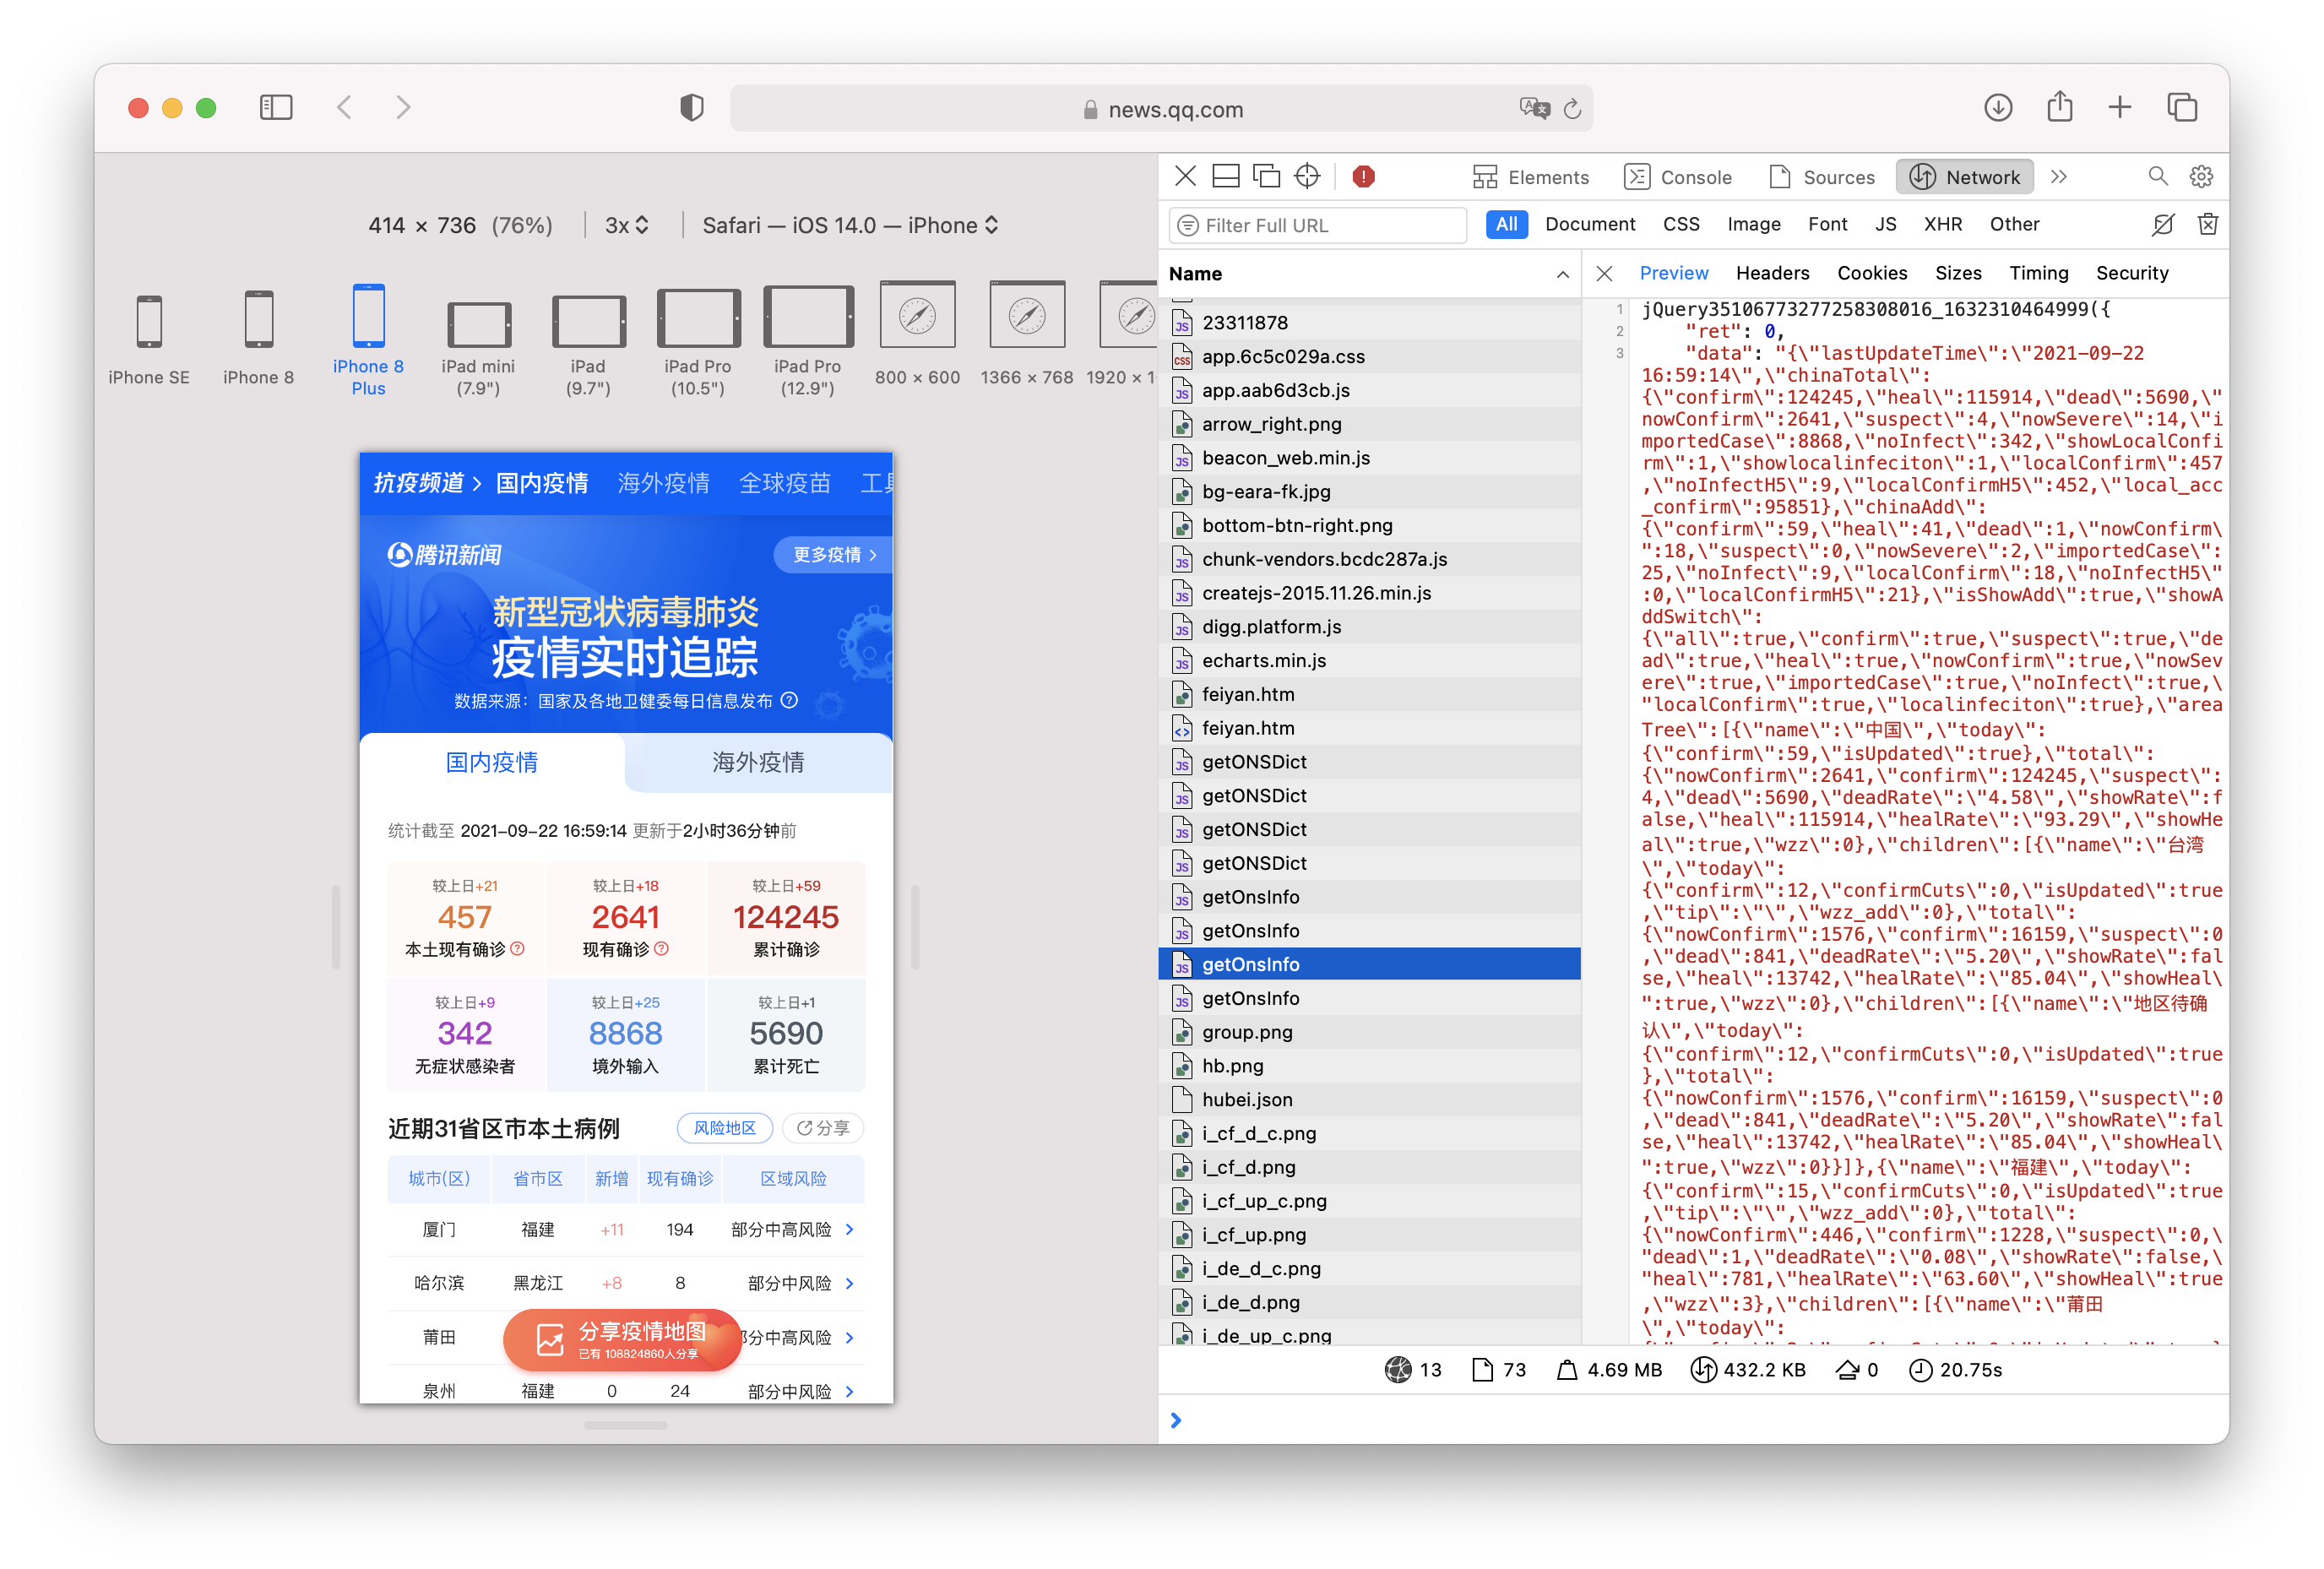
\includegraphics[width=0.8\textwidth]{t3}
    \bicaption{查看腾讯新闻疫情数据网站network情况}{Check Tencent News Epidemic Data Website Network Status}
    \label{fig:t3}
\end{figure}

之后,使用Python的requests库请求数据接口,然后解析json数据,将数据转换为字典类型,代码如下。

\lstset{
 columns=fixed,       
 numbers=left,                                        % 在左侧显示行号
 numberstyle=\tiny\color{gray},                       % 设定行号格式
 frame=none,                                          % 不显示背景边框
 backgroundcolor=\color[RGB]{245,245,244},            % 设定背景颜色
 keywordstyle=\color[RGB]{40,40,255},                 % 设定关键字颜色
 numberstyle=\footnotesize\color{darkgray},           
 commentstyle=\it\color[RGB]{0,96,96},                % 设置代码注释的格式
 stringstyle=\rmfamily\slshape\color[RGB]{128,0,0},   % 设置字符串格式
 showstringspaces=false,                              % 不显示字符串中的空格
 language=Python,                                        % 设置语言
}
\begin{lstlisting}
    def get_tencent_data():
    url = 'https://view.inews.qq.com/g2/getOnsInfo?name=disease_h5'
    url_his = 'https://view.inews.qq.com/g2/getOnsInfo?name=disease_other'
    headers = {
        'user-agent': 'Mozilla/5.0 (Windows NT 10.0; Win64; x64) AppleWebKit/537.36 (KHTML, like Gecko) Chrome/65.0.3325.181 Safari/537.36',
    }

    r = requests.get(url, headers)
    res = json.loads(r.text)  # json字符串转字典
    data_all = json.loads(res['data'])

    r_his = requests.get(url_his, headers)
    res_his = json.loads(r_his.text)
    data_his = json.loads(res_his['data'])

    history = {}  # 历史数据
\end{lstlisting}

r的键值为ret,data,其中ret为响应值,0为请求成功,data则是我们所需要的数据。使用json库将data转为字典类型,对数据进行一些处理之后,存入数据库。


\begin{lstlisting}
    for i in data_his["chinaDayList"]:
        ds = "2020." + i["date"]
        tup = time.strptime(ds, "%Y.%m.%d")
        ds = time.strftime("%Y-%m-%d", tup)  # 改变时间格式
        confirm = i["confirm"]
        suspect = i["suspect"]
        heal = i["heal"]
        dead = i["dead"]
        history[ds] = {"confirm": confirm, "suspect": suspect, "heal": heal, "dead": dead}
    for i in data_his["chinaDayAddList"]:
        ds = "2020." + i["date"]
        tup = time.strptime(ds, "%Y.%m.%d")
        ds = time.strftime("%Y-%m-%d", tup)
        confirm = i["confirm"]
        suspect = i["suspect"]
        heal = i["heal"]
        dead = i["dead"]
        history[ds].update({"confirm_add": confirm, "suspect_add": suspect, "heal_add": heal, "dead_add": dead})
\end{lstlisting}

将爬取到的json数据转换为字典类型并存入到histoty与details中。

\begin{lstlisting}
    def update_details():
    """
    更新 details 表
    :return:
    """
    cursor = None
    conn = None
    try:
        li = get_tencent_data()[1]  # 0 是历史数据字典,1 最新详细数据列表
        conn, cursor = get_conn()
        sql = """insert into details(update_time,province,city,confirm,confirm_add,heal,dead) values(%s,%s,%s,%s,%s,%s,%s)"""
        sql_query = """select %s='(select update_time from details order by id desc limit 1)'"""  # 对比当前最大时间戳
        cursor.execute(sql_query, li[0][0])
        if not cursor.fetchone()[0]:
            print(f"{time.asctime()}开始更新最新数据")
            for item in li:
                cursor.execute(sql, item)
            conn.commit()  # 提交事务 update delete insert操作
            print(f"{time.asctime()}更新最新数据完毕")
        else:
            print(f"{time.asctime()}已是最新数据!")
    except:
        traceback.print_exc()
    finally:
        close_conn(conn, cursor)
\end{lstlisting}

\section{数据的存储}

本系统所用到MySQL数据库为cov,内含history与details两个表,history用于存放过去三十天的疫情数据,detail用来存放今日国内疫情数据,其各自结构如下所示。

\begin{lstlisting}
  mysql> desc history;
  +-------------+------+------+-----+---------+-------+
  | Field       | Type | Null | Key | Default | Extra |
  +-------------+------+------+-----+---------+-------+
  | ds          | date | YES  |     | NULL    |       |
  | confirm     | int  | YES  |     | NULL    |       |
  | suspect     | int  | YES  |     | NULL    |       |
  | heal        | int  | YES  |     | NULL    |       |
  | dead        | int  | YES  |     | NULL    |       |
  | confirm_add | int  | YES  |     | NULL    |       |
  | suspect_add | int  | YES  |     | NULL    |       |
  | heal_add    | int  | YES  |     | NULL    |       |
  | dead_add    | int  | YES  |     | NULL    |       |
  +-------------+------+------+-----+---------+-------+
  9 rows in set (0.00 sec)
  
  mysql> desc details;
  +-------------+-------------+------+-----+---------+-------+
  | Field       | Type        | Null | Key | Default | Extra |
  +-------------+-------------+------+-----+---------+-------+
  | update_time | date        | YES  |     | NULL    |       |
  | province    | varchar(25) | YES  |     | NULL    |       |
  | city        | varchar(25) | YES  |     | NULL    |       |
  | confirm     | int         | YES  |     | NULL    |       |
  | confirm_add | int         | YES  |     | NULL    |       |
  | heal        | int         | YES  |     | NULL    |       |
  | dead        | int         | YES  |     | NULL    |       |
  +-------------+-------------+------+-----+---------+-------+
  7 rows in set (0.00 sec)
\end{lstlisting}

创建与关闭数据库连接。

\begin{lstlisting}
    def get_conn():
    """
    :return: 连接,游标
    """
    # 创建连接
    conn = pymysql.connect(host="127.0.0.1",
                           user="root",
                           password="123456",
                           db="cov",
                           charset="utf8")
    # 创建游标
    cursor = conn.cursor()  # 执行完毕返回的结果集默认以元组显示
    return conn, cursor


def close_conn(conn, cursor):
    if cursor:
        cursor.close()
    if conn:
        conn.close()
\end{lstlisting}



\chapter{网页设计}

\section{主页(index.html)的设计}

Html部分较为清晰简单,主页上部设计一列导航栏,主体部分分为左中右三个大部分,每个大部分分为两个小部分,后期将使用Echarts绘制图表并进行响应式布局。

\lstset{
 columns=fixed,       
 numbers=left,                                        % 在左侧显示行号
 numberstyle=\tiny\color{gray},                       % 设定行号格式
 frame=none,                                          % 不显示背景边框
 backgroundcolor=\color[RGB]{245,245,244},            % 设定背景颜色
 keywordstyle=\color[RGB]{40,40,255},                 % 设定关键字颜色
 numberstyle=\footnotesize\color{darkgray},           
 commentstyle=\it\color[RGB]{0,96,96},                % 设置代码注释的格式
 stringstyle=\rmfamily\slshape\color[RGB]{128,0,0},   % 设置字符串格式
 showstringspaces=false,                              % 不显示字符串中的空格
 language=html,                                        % 设置语言
}
\begin{lstlisting}
    <div class="row-cols-md-4 row">
        <div id="l1">我是左1</div>
        <div id="l2">我是左2</div>
    </div>
    <div class="row-cols-md-4 row">
        <div id="c1" class="row clearfix">
            <div class="txt"><h2 class="text-lg-center text-center">累计确诊</h2></div>
            <div class="txt"><h2 class="text-lg-center text-center">剩余疑似</h2></div>
            <div class="txt"><h2 class="text-lg-center text-center">累计治愈</h2></div>
            <div class="txt"><h2 class="text-lg-center text-center">累计死亡</h2></div>
            <div class="num"><h1 class="text-primary text-center"></h1></div>
            <div class="num"><h1 class="text-primary text-center"></h1></div>
            <div class="num"><h1 class="text-primary text-center"></h1></div>
            <div class="num"><h1 class="text-primary text-center"></h1></div>
        </div>
        <div id="c2">我是中2</div>
    </div>
    <div class="row-cols-md-4 row">
        <div id="r1">我是右1</div>
        <div id="r2">我是右2</div>
    </div>
\end{lstlisting}

\section{数据可视化}

为了使得该系统在不同屏幕尺寸的设备上能够正确显示,按照Bootstrap框架对前端网页进行构建。页面顶部为导航栏(navbar navbar-default),作为不同功能分区以及后续更多功能的入口,右端搜索接口接入百度搜索,提供更为丰富的搜索功能。页面主体分为三个大部分,其中包括六个小部分,并按从左到右排列,每个div的id依次记为l1,l2,c1,c2,r1,r2。对于每一个列,其div的class设置为row-cols-md-4 row,以实现响应式布局。左上角l1为全国累计趋势曲线表,使用ECharts库以实现绘制。因为纵轴所表示的两个数值差距过大,l1与l2使用两个y轴绘制,并使用不同颜色加以区分。

在utils.py中,定义了每个div获取数据的方法,例如getunderline{~}l1underline{~}data,通过调用utils.py中的方法,从而连接到数据库并获得每个div所需的数据data。在controller.js中定义了数据在图表中的显示形式。

\begin{figure}[H]
    \centering
    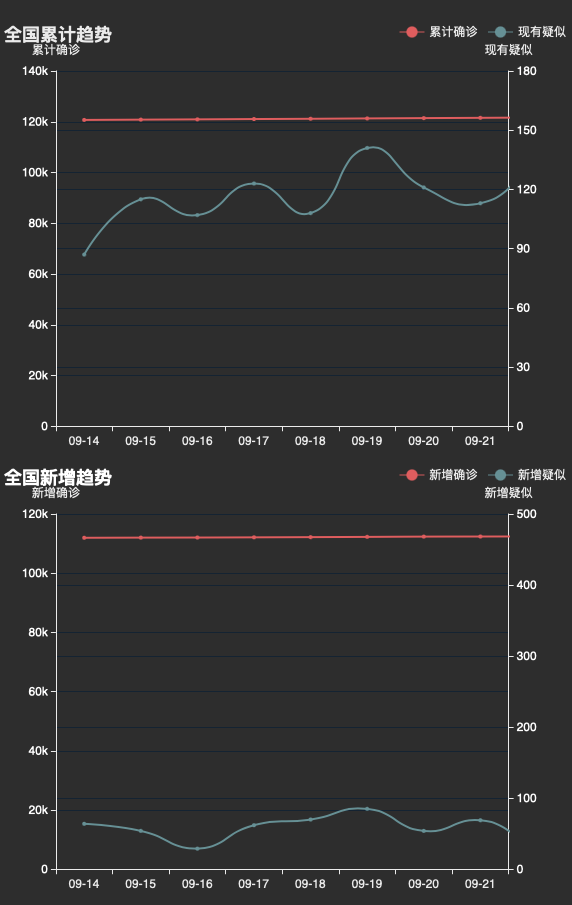
\includegraphics[width=0.8\textwidth]{t4}
    \bicaption{全国累计趋势与新增趋势}{National cumulative trends and new trends}
    \label{fig:t4}
\end{figure}

中上数据统计部分,使用类选择器显示当前累计确诊、剩余疑似、累计治愈以及累计死亡数据。

\lstset{
 columns=fixed,       
 numbers=left,                                        % 在左侧显示行号
 numberstyle=\tiny\color{gray},                       % 设定行号格式
 frame=none,                                          % 不显示背景边框
 backgroundcolor=\color[RGB]{245,245,244},            % 设定背景颜色
 keywordstyle=\color[RGB]{40,40,255},                 % 设定关键字颜色
 numberstyle=\footnotesize\color{darkgray},           
 commentstyle=\it\color[RGB]{0,96,96},                % 设置代码注释的格式
 stringstyle=\rmfamily\slshape\color[RGB]{128,0,0},   % 设置字符串格式
 showstringspaces=false,                              % 不显示字符串中的空格
 language=html,                                        % 设置语言
}
\begin{lstlisting}
    function get_c1_data() {
    $.ajax({
        url: "/c1",
        success: function (data) {
            $(".num h1").eq(0).text(data.confirm);
            console.log(data.confirm);
            $(".num h1").eq(1).text(data.suspect);
            $(".num h1").eq(2).text(data.heal);
            $(".num h1").eq(3).text(data.dead);
        },
        error: function (xhr, type, errorThrown) {

        }
    })
}
\end{lstlisting}


\section{对手机设备的适配}

为了使得该系统可以在手机设备上显示,在main.css中加入了旋转屏幕的样式。当屏幕尺寸判断为竖屏时,将旋转页面,使其变为横屏。

\begin{lstlisting}
    @media screen and (orientation: portrait) {
        html{
            width : 100vmin;
            height : 100vmax;
        }
        body{
            width : 100vmin;
            height : 100vmax;
        }
        #gyroContain{
            width : 100vmax;
            height : 100vmin;
            transform-origin: top left;
            transform: rotate(90deg) translate(0,-100vmin);
        }
      }
    @media screen and (orientation: landscape) {
        html{
            width : 100vmax;
            height : 100vmin;
        }
        body{
            width : 100vmax;
            height : 100vmin;
        }
        #gyroContain{
            width : 100vmax;
            height : 100vmin;
        }
    }
\end{lstlisting}







% \chapter{\LaTeX{}使用说明}\label{chap:guide}

为方便使用及更好地展示\LaTeX{}排版的优秀特性,ucasthesis的框架和文件体系进行了细致地处理,尽可能地对各个功能和板块进行了模块化和封装,对于初学者来说,众多的文件目录也许一开始让人觉得有些无所适从,但阅读完下面的使用说明后,会发现原来使用思路是简单而清晰的,而且,当对\LaTeX{}有一定的认识和了解后,会发现其相对Word类排版系统极具吸引力的优秀特性。所以,如果是初学者,请不要退缩,请稍加尝试和坚持,以领略到\LaTeX{}的非凡魅力,并可以通过阅读相关资料如\LaTeX{} Wikibook \citep{杨晨2021新冠肺炎疫情大数据可视化平台设计与实现} 来完善自己的使用知识。

\section{先试试效果}
\citep{grinberg2018flask}
%---------------------------------------------------------------------------%
% main content
%-
%-> Appendix
%-
\cleardoublepage%
\appendix% initialize the environment
\chapter{Python代码}

\section{spider.py---用来爬取网页数据}

\lstset{
 columns=fixed,       
 numbers=left,                                        % 在左侧显示行号
 numberstyle=\tiny\color{gray},                       % 设定行号格式
 frame=none,                                          % 不显示背景边框
 backgroundcolor=\color[RGB]{245,245,244},            % 设定背景颜色
 keywordstyle=\color[RGB]{40,40,255},                 % 设定关键字颜色
 numberstyle=\footnotesize\color{darkgray},           
 commentstyle=\it\color[RGB]{0,96,96},                % 设置代码注释的格式
 stringstyle=\rmfamily\slshape\color[RGB]{128,0,0},   % 设置字符串格式
 showstringspaces=false,                              % 不显示字符串中的空格
 language=Python,                                        % 设置语言
}
\begin{lstlisting}
import os
import pymysql
import time
import json
import traceback  # 追踪异常
import requests


def get_tencent_data():
    url = 'https://view.inews.qq.com/g2/getOnsInfo?name=disease_h5'
    url_his = 'https://view.inews.qq.com/g2/getOnsInfo?name=disease_other'
    headers = {
        'user-agent': 'Mozilla/5.0 (Windows NT 10.0; Win64; x64) AppleWebKit/537.36 (KHTML, like Gecko) Chrome/65.0.3325.181 Safari/537.36',
    }

    r = requests.get(url, headers)
    res = json.loads(r.text)  # json字符串转字典
    data_all = json.loads(res['data'])

    r_his = requests.get(url_his, headers)
    res_his = json.loads(r_his.text)
    data_his = json.loads(res_his['data'])

    history = {}  # 历史数据

    for i in data_his["chinaDayList"]:
        ds = "2020." + i["date"]
        tup = time.strptime(ds, "%Y.%m.%d")
        ds = time.strftime("%Y-%m-%d", tup)  # 改变时间格式
        confirm = i["confirm"]
        suspect = i["suspect"]
        heal = i["heal"]
        dead = i["dead"]
        history[ds] = {"confirm": confirm, "suspect": suspect, "heal": heal, "dead": dead}
    for i in data_his["chinaDayAddList"]:
        ds = "2020." + i["date"]
        tup = time.strptime(ds, "%Y.%m.%d")
        ds = time.strftime("%Y-%m-%d", tup)
        confirm = i["confirm"]
        suspect = i["suspect"]
        heal = i["heal"]
        dead = i["dead"]
        history[ds].update({"confirm_add": confirm, "suspect_add": suspect, "heal_add": heal, "dead_add": dead})

    # 下面就不用动了
    details = []  # 当日详细数据
    update_time = data_all["lastUpdateTime"]
    data_country = data_all["areaTree"]  # list 25个国家
    data_province = data_country[0]["children"]  # 中国各省
    for pro_infos in data_province:
        province = pro_infos["name"]  # 省名
        for city_infos in pro_infos["children"]:
            city = city_infos["name"]
            confirm = city_infos["total"]["confirm"]
            confirm_add = city_infos["today"]["confirm"]
            heal = city_infos["total"]["heal"]
            dead = city_infos["total"]["dead"]
            details.append([update_time, province, city, confirm, confirm_add, heal, dead])
    return history, details


def get_conn():
    """
    :return: 连接,游标
    """
    # 创建连接
    conn = pymysql.connect(host="127.0.0.1",
                           user="root",
                           password="123456",
                           db="cov",
                           charset="utf8")
    # 创建游标
    cursor = conn.cursor()  # 执行完毕返回的结果集默认以元组显示
    return conn, cursor


def close_conn(conn, cursor):
    if cursor:
        cursor.close()
    if conn:
        conn.close()


def update_details():
    """
    更新 details 表
    :return:
    """
    cursor = None
    conn = None
    try:
        li = get_tencent_data()[1]  # 0 是历史数据字典,1 最新详细数据列表
        conn, cursor = get_conn()
        sql = """insert into details(update_time,province,city,confirm,confirm_add,heal,dead) values(%s,%s,%s,%s,%s,%s,%s)"""
        sql_query = """select %s='(select update_time from details order by id desc limit 1)'"""  # 对比当前最大时间戳
        cursor.execute(sql_query, li[0][0])
        if not cursor.fetchone()[0]:
            print(f"{time.asctime()}开始更新最新数据")
            for item in li:
                cursor.execute(sql, item)
            conn.commit()  # 提交事务 update delete insert操作
            print(f"{time.asctime()}更新最新数据完毕")
        else:
            print(f"{time.asctime()}已是最新数据!")
    except:
        traceback.print_exc()
    finally:
        close_conn(conn, cursor)


def insert_history():
    """
        插入历史数据
    :return:
    """
    cursor = None
    conn = None
    try:
        dic = get_tencent_data()[0]  # 0 是历史数据字典,1 最新详细数据列表
        print(f"{time.asctime()}开始插入历史数据")
        conn, cursor = get_conn()
        sql = """insert into history values(%s,%s,%s,%s,%s,%s,%s,%s,%s)"""
        for k, v in dic.items():
            # item 格式 {'2020-01-13': {'confirm': 41, 'suspect': 0, 'heal': 0, 'dead': 1}
            cursor.execute(sql, [k, v.get("confirm"), v.get("confirm_add"), v.get("suspect"),
                                 v.get("suspect_add"), v.get("heal"), v.get("heal_add"),
                                 v.get("dead"), v.get("dead_add")])

        conn.commit()  # 提交事务 update delete insert操作
        print(f"{time.asctime()}插入历史数据完毕")
    except:
        traceback.print_exc()
    finally:
        close_conn(conn, cursor)


def update_history():
    """
    更新历史数据
    :return:
    """
    cursor = None
    conn = None
    try:
        dic = get_tencent_data()[0]  # 0 是历史数据字典,1 最新详细数据列表
        print(f"{time.asctime()}开始更新历史数据")
        conn, cursor = get_conn()
        sql = """insert into history (ds,confirm,suspect,heal,dead,confirm_add,suspect_add,heal_add,dead_add) values(%s,%s,%s,%s,%s,%s,%s,%s,%s)"""
        sql_query = """select confirm from history where ds=%s"""
        for k, v in dic.items():
            # item 格式 {'2020-01-13': {'confirm': 41, 'suspect': 0, 'heal': 0, 'dead': 1}}
            if not cursor.execute(sql_query, k):
                cursor.execute(sql, [k, v.get("confirm"), v.get("confirm_add"), v.get("suspect"),
                                     v.get("suspect_add"), v.get("heal"), v.get("heal_add"),
                                     v.get("dead"), v.get("dead_add")])
        conn.commit()  # 提交事务 update delete insert操作
        print(f"{time.asctime()}历史数据更新完毕")
    except:
        traceback.print_exc()
    finally:
        close_conn(conn, cursor)


if __name__ == "__main__":
    insert_history()
    update_history()
    update_details()
\end{lstlisting}

\section{utils.py---app.py中所调用的方法}

\begin{lstlisting}
    import time
    import pymysql
    from decimal import Decimal
    import json
    
    
    def get_time():
        time_str = time.strftime("%Y{}%m{}%d{} %X")
        return time_str.format("年", "月", "日")
    
    
    def get_conn():
        """
        :return: 连接,游标
        """
        # 创建连接
        conn = pymysql.connect(host="localhost",
                               user="root",
                               password="123456",
                               db="cov",
                               charset="utf8")
        # 创建游标
        cursor = conn.cursor()  # 执行完毕返回的结果集默认以元组显示
        return conn, cursor
    
    
    def close_conn(conn, cursor):
        cursor.close()
        conn.close()
    
    
    def query(sql, *args):
        """
        封装通用查询
        :param sql:
        :param args:
        :return: 返回查询到的结果,((),(),)的形式
        """
        conn, cursor = get_conn()
        cursor.execute(sql, args)
        res = cursor.fetchall()
        close_conn(conn, cursor)
        return res
    
    
    def get_c1_data():
        """
        :return: 返回大屏div id=c1 的数据
        """
        # 因为会更新多次数据,取时间戳最新的那组数据
        sql = "select sum(confirm)," \
              "(select suspect from history order by ds desc limit 1)," \
              "sum(heal)," \
              "sum(dead) " \
              "from details " \
              "where update_time=(select update_time from details order by update_time desc limit 1) "
              #"where update_time=(select update_time from details order by update_time desc limit 1) "
        res = query(sql)
    
        res_list = [str(i) for i in res[0]]
        res_tuple = tuple(res_list)
        return res_tuple
    
    
    def get_c2_data():
        """
        :return:  返回各省数据
        """
        # 因为会更新多次数据,取时间戳最新的那组数据
        sql = "select province,sum(confirm) from details " \
              "where update_time=(select update_time from details " \
              "order by update_time desc limit 1) " \
              "group by province"
        res = query(sql)
        return res
    
    
    def get_l1_data():
        sql = "select ds,confirm,suspect,heal,dead from history"
        res = query(sql)
        return res
    
    
    def get_l2_data():
        sql = "select ds,confirm_add,suspect_add from history"
        res = query(sql)
        return res
    
    
    def get_r1_data():
        """
        :return:  返回非湖北地区城市确诊人数前5名
        """
        sql = 'SELECT province,confirm_add FROM ' \
              '(select province,sum(confirm_add) as confirm_add from details  ' \
              'where update_time=(select update_time from details order by update_time desc limit 1) ' \
              'group by province) as a ' \
              'ORDER BY confirm_add DESC LIMIT 5'
        res = query(sql)
        return res
    
    
    def get_r2_data():
        '''
            获取世界各国的疫情数据
            :return:
        '''
        # 因为会更新多次数据,取时间戳最新的那组数据
        sql = "select province,sum(confirm_add) from details " \
              "where update_time=(select update_time from details " \
              "order by update_time desc limit 1) " \
              "group by province"
        res = query(sql)
        return res
    
    
    if __name__ == "__main__":
        print(get_c1_data())
\end{lstlisting}    

\section{app.py---启动Flask的主程序}

\begin{lstlisting}
    import utils
    from flask import Flask
    from flask import request
    from flask import render_template
    from flask import jsonify
    from flask_bootstrap import Bootstrap
    import os
    import string
    
    os.system(
        'python3 /Users/liuhaoxin/Documents/GitHub/covid-19-china/spider.py && python3 /Users/liuhaoxin/Documents/GitHub/covid-19-china/utils.py')
    
    app = Flask(__name__)
    bootstrap = Bootstrap(app)
    
    @app.route('/')
    def hello_world():
        return render_template("index.html")
    
    
    @app.route("/c1")
    def get_c1_data():
        data = utils.get_c1_data()
        return jsonify({"confirm":data[0],"suspect":data[1],"heal":data[2],"dead":data[3]})
    
    
    @app.route("/c2")
    def get_c2_data():
        res = []
        for tup in utils.get_c2_data():
            # print(tup)
            res.append({"name":tup[0],"value":int(tup[1])})
        return jsonify({"data":res})
    
    
    @app.route("/l1")
    def get_l1_data():
        data = utils.get_l1_data()
        day,confirm,suspect,heal,dead = [],[],[],[],[]
        for a,b,c,d,e in data[7:]:
            day.append(a.strftime("%m-%d"))
            #  a是datatime类型
            confirm.append(b)
            suspect.append(c)
            heal.append(d)
            dead.append(e)
        return jsonify({"day": day, "confirm": confirm, "suspect": suspect, "heal": heal, "dead": dead})
    
    
    @app.route("/l2")
    def get_l2_data():
        data = utils.get_l2_data()
        day, confirm_add, suspect_add = [], [], []
        for a, b, c in data[7:]:
            day.append(a.strftime("%m-%d"))  # a是datatime类型
            confirm_add.append(b)
            suspect_add.append(c)
        return jsonify({"day": day, "confirm_add": confirm_add, "suspect_add": suspect_add})
    
    
    @app.route("/r1")
    def get_r1_data():
        data = utils.get_r1_data()
        city = []
        confirm = []
        for k,v in data:
            city.append(k)
            confirm.append(int(v))
        return jsonify({"city": city, "confirm": confirm})
    
    
    @app.route("/r2")
    def get_r2_data():
        res = []
        for tup in utils.get_r2_data():
            # print(tup)
            res.append({"name": tup[0], "value": int(tup[1])})
        return jsonify({"data": res})
    
    
    @app.route("/time")
    def get_time():
        return utils.get_time()
    
    
    if __name__ == '__main__':
        # app.run(host='127.0.0.1', port=5000)
        bootstrap.run()
\end{lstlisting}

\chapter{网页代码}

\section{index.html}

\lstset{
 columns=fixed,       
 numbers=left,                                        % 在左侧显示行号
 numberstyle=\tiny\color{gray},                       % 设定行号格式
 frame=none,                                          % 不显示背景边框
 backgroundcolor=\color[RGB]{245,245,244},            % 设定背景颜色
 keywordstyle=\color[RGB]{40,40,255},                 % 设定关键字颜色
 numberstyle=\footnotesize\color{darkgray},           
 commentstyle=\it\color[RGB]{0,96,96},                % 设置代码注释的格式
 stringstyle=\rmfamily\slshape\color[RGB]{128,0,0},   % 设置字符串格式
 showstringspaces=false,                              % 不显示字符串中的空格
 language=html,                                        % 设置语言
}
\begin{lstlisting}
    <!DOCTYPE html>
    <html>
    <head>
        <meta charset="utf-8">
        <meta http-equiv="X-UA-Compatible" content="IE=edge">
        <meta name="viewport" content="width=device-width, initial-scale=1.0">
        <title>疫情监控系统</title>
        <link rel="icon" href="../static/icon.ico">
        <link rel="stylesheet" href="https://cdn.staticfile.org/twitter-bootstrap/3.3.7/css/bootstrap.min.css">
        <script src="https://cdn.staticfile.org/jquery/2.1.1/jquery.min.js"></script>
        <script src="https://cdn.staticfile.org/twitter-bootstrap/3.3.7/js/bootstrap.min.js"></script>
        <script src="../static/js/jquery-1.11.1.min.js"></script>
        <script src="../static/js/echarts.min.js"></script>
        <script src="../static/js/china.js"></script>
        <link href="../static/css/main.css" rel="stylesheet"/>
    </head>
    <body>
    
    <div id="tim"></div>
    <div id="gyroContain" class="col clearfix">
        <div class="row clearfix">
            <div class="col-md-12 column">
                <nav class="navbar navbar-default" role="navigation">
                    <div class="navbar-header">
                        <a class="navbar-brand" href="#">疫情数据监控平台</a>
                    </div>
    
                    <div class="collapse navbar-collapse" id="bs-example-navbar-collapse-1">
                        <ul class="nav navbar-nav">
                            <li class="active">
                                <a href="#">国内数据</a>
                            </li>
                            <li>
                                <a href="#">国外数据</a>
                            </li>
                            <li class="dropdown">
                                <a href="#" class="dropdown-toggle" data-toggle="dropdown">更多<strong
                                        class="caret"></strong></a>
                                <ul class="dropdown-menu">
                                    <li>
                                        <a href="https://www.baidu.com/#ie=utf8&wd=疫情最新政策">最新政策</a>
                                    </li>
                                    <li>
                                        <a href="https://www.baidu.com/#ie=utf8&wd=疫情当地政策">当地政策</a>
                                    </li>
                                    <li>
                                        <a href="https://www.baidu.com/#ie=utf8&wd=疫情国际消息">国际消息</a>
                                    </li>
                                    <li class="divider">
                                    </li>
                                    <li>
                                        <a href="#">健康码</a>
                                    </li>
                                    <li class="divider">
                                    </li>
                                    <li>
                                        <a href="#">防疫平台</a>
                                    </li>
                                </ul>
                            </li>
                        </ul>
    
                        <ul class="nav navbar-nav navbar-right">
                            <form class="navbar-form navbar-left" role="search">
                                <div class="form-group">
                                    <input type="text" class="form-control"/>
                                </div>
                                <button type="submit" class="btn btn-default">搜索</button>
                            </form>
                        </ul>
                    </div>
    
                </nav>
            </div>
        </div>
        <div class="row-cols-md-4 row">
            <div id="l1">我是左1</div>
            <div id="l2">我是左2</div>
        </div>
        <div class="row-cols-md-4 row">
            <div id="c1" class="row clearfix">
                <div class="txt"><h2 class="text-lg-center text-center">累计确诊</h2></div>
                <div class="txt"><h2 class="text-lg-center text-center">剩余疑似</h2></div>
                <div class="txt"><h2 class="text-lg-center text-center">累计治愈</h2></div>
                <div class="txt"><h2 class="text-lg-center text-center">累计死亡</h2></div>
                <div class="num"><h1 class="text-primary text-center"></h1></div>
                <div class="num"><h1 class="text-primary text-center"></h1></div>
                <div class="num"><h1 class="text-primary text-center"></h1></div>
                <div class="num"><h1 class="text-primary text-center"></h1></div>
            </div>
            <div id="c2">我是中2</div>
        </div>
        <div class="row-cols-md-4 row">
            <div id="r1">我是右1</div>
            <div id="r2">我是右2</div>
        </div>
    
        <script src="../static/js/ec_center.js"></script>
        <script src="../static/js/ec_left1.js"></script>
        <script src="../static/js/ec_left2.js"></script>
        <script src="../static/js/ec_right1.js"></script>
        <script src="../static/js/ec_right2.js"></script>
        <script src="../static/js/controller.js"></script>
    </div>
    </body>
    </html>
\end{lstlisting}

\section{controller.js}
\begin{lstlisting}
    function gettime() {
        $.ajax({
            url: "/time",
            timeout: 10000, //超时时间设置为10秒;
            success: function (data) {
                $("#tim").html(data)
            },
            error: function (xhr, type, errorThrown) {
    
            }
        });
    }
    
    function get_c1_data() {
        $.ajax({
            url: "/c1",
            success: function (data) {
                $(".num h1").eq(0).text(data.confirm);
                console.log(data.confirm);
                $(".num h1").eq(1).text(data.suspect);
                $(".num h1").eq(2).text(data.heal);
                $(".num h1").eq(3).text(data.dead);
            },
            error: function (xhr, type, errorThrown) {
    
            }
        })
    }
    
    function get_c2_data() {
        $.ajax({
            url: "/c2",
            success: function (data) {
                ec_center_option.series[0].data = data.data
                ec_center.setOption(ec_center_option)
            },
            error: function (xhr, type, errorThrown) {
    
            }
        })
    }
    
    function get_l1_data() {
        $.ajax({
            url: "/l1",
            success: function (data) {
                var day = []
                for (let i = 0; i < 8; i++) {
                    day[7 - i] = data.day[data.day.length - 1 - i]
                }
                // ec_left1_Option.xAxis[0].data=data.day
                ec_left1_Option.xAxis[0].data = day
                ec_left1_Option.series[0].data = data.confirm
                console.log(data.confirm);
                ec_left1_Option.series[1].data = data.suspect
                // ec_left1_Option.series[2].data = data.heal
                // ec_left1_Option.series[3].data = data.dead
                ec_left1.setOption(ec_left1_Option)
                // console.log(day)
            },
            error: function (xhr, type, errorThrown) {
    
            }
        })
    }
    
    function get_l2_data() {
        $.ajax({
            url: "/l2",
            success: function (data) {
                var day = []
                for (let i = 0; i < 8; i++) {
                    day[7 - i] = data.day[data.day.length - 1 - i]
                }
                ec_left2_Option.xAxis[0].data = day
                ec_left2_Option.series[0].data = data.confirm_add
                ec_left2_Option.series[1].data = data.suspect_add
                ec_left2.setOption(ec_left2_Option)
            },
            error: function (xhr, type, errorThrown) {
    
            }
        })
    }
    
    function get_r1_data() {
        $.ajax({
            url: "/r1",
            success: function (data) {
                ec_right1_option.xAxis.data = data.city;
                ec_right1_option.series[0].data = data.confirm;
                ec_right1.setOption(ec_right1_option);
            }
        })
    }
    
    function get_r2_data() {
        $.ajax({
            url: "/r2",
            success: function (data) {
                ec_right2_option.series[0].data = data.data
                ec_right2.setOption(ec_right2_option)
    
            },
            error: function (xhr, type, errorThrown) {
    
            }
        })
    }
    
    gettime()
    get_c1_data()
    get_c2_data()
    get_l1_data()
    get_l2_data()
    get_r1_data()
    get_r2_data()
    
    setInterval(gettime, 1000)
    setInterval(get_c1_data, 1000 * 10)
    setInterval(get_c2_data, 10000 * 10)
    setInterval(get_l1_data, 10000 * 10)
    setInterval(get_l2_data, 10000 * 10)
    setInterval(get_r1_data, 10000 * 10)
    setInterval(get_r2_data, 10000 * 10)
\end{lstlisting}

\section{ec\underline{~}center.js}
\begin{lstlisting}
    var ec_center = echarts.init(document.getElementById('c2'), "dark");

    var mydata = []
    
    var ec_center_option = {
        title: {
            text: '全国累计确诊地图',
            subtext: '',
            x: 'center'
        },
        tooltip: {
            trigger: 'item'
        },
        //左侧小导航图标
        visualMap: {
            show: true,
            x: 'left',
            y: 'bottom',
            textStyle: {
                fontSize: 8,
            },
            splitList: [{ start: 1,end: 9 },
                {start: 10, end: 99 }, 
                { start: 100, end: 999 },
                {  start: 1000, end: 9999 },
                { start: 10000 }],
            color: ['#8A3310', '#C64918', '#E55B25', '#F2AD92', '#F9DCD1']
        },
        //配置属性
        series: [{
            name: '累计确诊人数',
            type: 'map',
            mapType: 'china',
            roam: false, //拖动和缩放
            itemStyle: {
                normal: {
                    borderWidth: .5, //区域边框宽度
                    borderColor: '#009fe8', //区域边框颜色
                    areaColor: "#ffefd5", //区域颜色
                },
                emphasis: { //鼠标滑过地图高亮的相关设置
                    borderWidth: .5,
                    borderColor: '#4b0082',
                    areaColor: "#fff",
                }
            },
            label: {
                normal: {
                    show: true, //省份名称
                    fontSize: 8,
                },
                emphasis: {
                    show: true,
                    fontSize: 8,
                }
            },
            data:[] //mydata //数据
        }]
    };
    ec_center.setOption(ec_center_option)
\end{lstlisting}


% appendix content
%-
%-> Backmatter: bibliography, glossary, index
%-
\backmatter% initialize the environment
\intotoc*{\cleardoublepage}{\bibname}% add link to toc
\artxifstreq{\artxbib}{bibtex}{% enable bibtex
    \bibliography{Biblio/ref}% bibliography
}{%
    \printbibliography% bibliography
}
% %---------------------------------------------------------------------------%
%->> Backmatter
%---------------------------------------------------------------------------%
\chapter[致谢]{致\quad 谢}\chaptermark{致\quad 谢}% syntax: \chapter[目录]{标题}\chaptermark{页眉}
%\thispagestyle{noheaderstyle}% 如果需要移除当前页的页眉
%\pagestyle{noheaderstyle}% 如果需要移除整章的页眉

行文至此,落笔为念。两年半前踏入大学的之日仿佛就在昨天,目光所到之处,每一间教室,每一个角落,皆是回忆。我将永远热爱那段在机房调试代码的时光,每一行代码,每一个数据都犹如眼睛,所到之处里尽是无限的灵感。

首先在此我要感谢我的导师王震教授,感谢他在本文写作过程中给出的意见与格式修改的建议。从开题到初稿再到定稿,老师都在给予无微不至指导与帮助。在老师身上我学到很多东西,对学术认真、一丝不苟的精神。这些收获将会令我受益终生,让我在未来的学习与工作中多一份信心与勇气。

借此机会,特别感谢我的父母。二十余载求学之路,离不开背后父母的默默付出。在我面对困难时,您永远是我最坚强的后盾,不断支持着我去追寻我所喜爱的事业。

除此之外,我还要提到一位特别重要的人——姚庆悦。青春兵荒马乱,我们潦草的离散,感谢你曾出现在我的生命中并陪我走过那段难忘的高中时光。

本文使用\LaTeX{}模版ucasthesis写作,在此特别感谢casthesis作者吴凌云学长,gbt7714-bibtex-style开发者zepinglee和ctex众多开发者们。尤其感谢GitHub项目ucasthesis作者莫晃锐的开源\LaTeX{}模版。在此对所有\LaTeX{}社区的贡献者表示感谢!

% \chapter{作者简历及攻读学位期间发表的学术论文与研究成果}

% \textbf{本科生无需此部分}。

% \section*{作者简历:}

% \subsection*{casthesis作者}

% 吴凌云,福建省屏南县人,中国科学院数学与系统科学研究院博士研究生。

% \subsection*{ucasthesis作者}

% 莫晃锐,湖南省湘潭县人,中国科学院力学研究所硕士研究生。

% \section*{已发表(或正式接受)的学术论文:}

% {
% \setlist[enumerate]{}% restore default behavior
% \begin{enumerate}[nosep]
%     \item ucasthesis: A LaTeX Thesis Template for the University of Chinese Academy of Sciences, 2014.
% \end{enumerate}
% }

% \section*{申请或已获得的专利:}

% (无专利时此项不必列出)

% \section*{参加的研究项目及获奖情况:}

% 可以随意添加新的条目或是结构。

\cleardoublepage[plain]% 让文档总是结束于偶数页,可根据需要设定页眉页脚样式,如 [noheaderstyle]
%---------------------------------------------------------------------------%
% other information
\end{document}
%---------------------------------------------------------------------------%

